

\documentclass[10pt,a4paper,twoside]{article}
\usepackage[dutch]{babel}
\usepackage{amssymb}
\usepackage{amsmath}
\usepackage{float,flafter}	
\usepackage{hyperref}
\usepackage{inputenc}
\usepackage{graphicx}
\setlength\paperwidth{20.999cm}\setlength\paperheight{29.699cm}\setlength\voffset{-1in}\setlength\hoffset{-1in}\setlength\topmargin{1cm}\setlength\headheight{12pt}\setlength\headsep{0cm}\setlength\footskip{1.131cm}\setlength\textheight{25cm}\setlength\oddsidemargin{2.499cm}\setlength\textwidth{15.999cm}
\begin{document}
\begin{center}
\vspace{.3cm}
{\bf {\huge Term paper}}
\item
{\bf {\huge ORM in DBMS}}
\vspace{.3cm}
\end{center}
{\bf Name:}  Bhavin Raichura\\
{\bf Roll no:}  19111019 \\
{\bf Subject:}  DBMS\\
{\bf Branch:}  Biomedical Engineering \hspace{\fill}   \\
\hrule

\vspace{.5cm}
\vspace{.4cm}

\renewcommand{\abstractname}{Abstract}

\begin{abstract}
\item One of the challenges of using object-oriented programming (OOP) languages and databases is the complexity of aligning the programming code with database structures. Object-relational mapping (ORM) is a technique that creates a layer between the language and the database, helping programmers work with data without the OOP paradigm.
\item The necessity to learn and code in structured query language (SQL) in order to link their application to a SQL database is a problem for OOP developers.
Data-access code can be written by developers who are familiar with SQL.
Because the developer must extract the data items from the code strings, this raw SQL coding might take a long time.To provide extra information about the data, SQL query builders provide a layer of abstraction to the SQL code. Developers, on the other hand, must be able to read and write SQL.
\item In this term paper I will provide an overview of ORMs, and compare them with SQL tools using an example of an database based application using python.
\end{abstract}

\item
\item
{\bf {\Large This term paper will highlight the following aspects:  }}\\
\begin{itemize}
\end{itemize}
\item 
\begin{enumerate}
\item Introduction: ORM
\item How ORM Works
\item Common Languages Between ORMs and OOPs
\item ORM vs Raw SQL
\item OOPs Concepts
\item Some Basic SQL Operations in ORM using SQLAlchemy 
\item Features
\item Pros of ORM
\item Cons of ORM
\item Conclusion
\item Reference 
\end{enumerate}

\section{Introduction: ORM}
\item An object-relational mapper provides an object-oriented layer between relational databases and object-oriented programming languages(like C++, C, Python, JAVA) without having to write SQL queries. It standardizes interfaces reducing boilerplate and speeding development time.
\item Object-oriented programming includes many states and codes in a format that is complex to understand and interpret. ORMs translate this data and create a structured map to help developers understand the underlying database structure. The mapping explains how objects are related to different tables. ORMs use this information to convert data between tables and generate the SQL code for a relational database to insert, update, create and delete data in response to changes the application makes to the data object. Once written, the ORM mapping will manage the application’s data needs and you will not need to write any more low-level code.


\section{How ORM Works}
It operates on the objects. So the whole methodology followed by ORMs is dependent on the object-oriented paradigm. ORMs generate objects which map to tables in the database virtually. It create a model of the object-oriented program with a high-level of abstraction. In other words, it makes a level of logic without the underlying details of the code. Mapping describes the relationship between an object and the data without knowing how the data is structured. The model can then be used to connect the application with the SQL code needed to manage data activities. This “plumbing” type of code does not have to be rewritten, saving the developer a tremendous amount of time.
\item
\begin{figure1}
  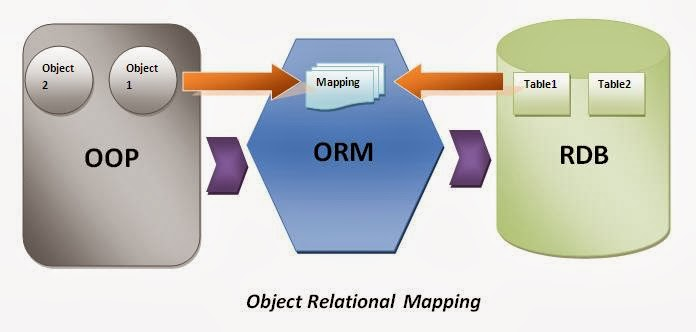
\includegraphics[width=\linewidth]{./images/orm1.JPG}
  \caption{Figure 1:Working of ORM}
  \label{fig:ORM}
\end{figure1}


\section{Common Languages Between ORMs and OOPs}
\begin{itemize}
\item  Hibernate: JAVA
\item     Django ORM: Django
\item     SQL Alchemy: Flask
\item     Dapper ORM: C\#
\item     JOOQ ORM: JAVA
\item     Doctrine: PHP
\end{itemize}


\section{ORM vs Raw SQL}
Developers can use raw SQL code to write a direct interface between the application and the database. Most relational databases support SQL to build data interfaces and applications. It’s stable, and since SQL has been used since the 1970s, it’s well documented and supported. Programmers maintain a lot of control over their data interface with SQL. It requires a lot of work, but it is more flexible and detailed than an ORM abstraction.
\item
\begin{figure2}
  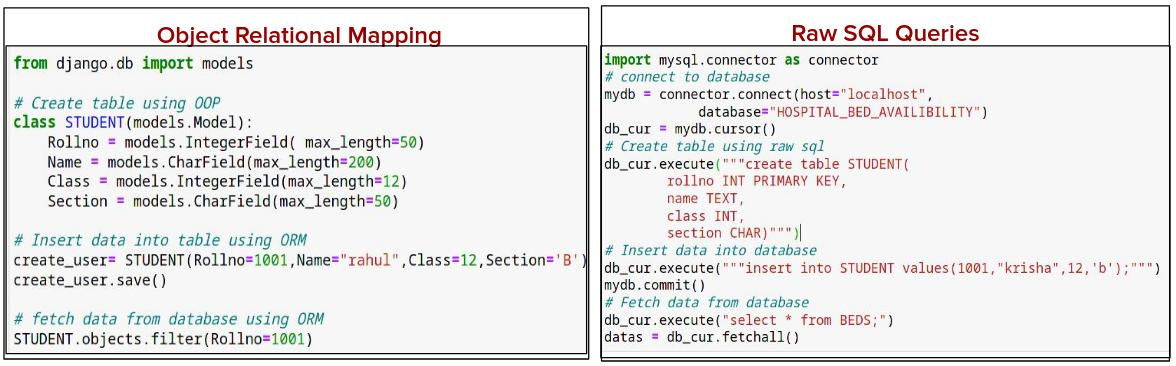
\includegraphics[width=\linewidth]{./images/orm2.jpg}
  \caption{Figure 2: ORM vs Raw SQL}
  \label{fig:ORM vs SQL}
\end{figure2}

\subsection{Native Querying with SQL}
\item Using raw SQL also has its drawbacks. For instance, the developer is responsible for the safety and security of the database code. SQL injection is a problem where user input can affect the data state causing issues with the application and data integrity. ORMs sanitizes the code, making it easier to avoid these problems.

\subsection{SQL Query Builders}
\item Query builders add a layer of abstraction over the raw SQL without masking all of the underlying details. The builders formalize querying patterns and add methods to or functions that add escape items for easier application integration. They add a templating layer to help developers understand the database structure within the same coding application. Template builders still require developers to understand the database structure, requiring them to know SQL.


\section{OOPs Concept}
\item Object oriented programming is a type of programming which uses objects and classes its functioning. The object oriented programming is based on real world entities like inheritance, polymorphism, data hiding, etc. It aims at binding together data and function work on these data sets into a single entity to restrict their usage.
\item Some basic concepts of object oriented programming are −
\begin{itemize}
\item     CLASS
\item     OBJECTS
\item     ENCAPSULATION
\item     POLYMORPHISM
\item     INHERITANCE
\item     ABSTRACTION
\end{itemize}

\subsection{Class} 
\item A class is a data-type that has its own members i.e. data members and member functions. It is the blueprint for an object in object oriented programming language. It is the basic building block of object oriented programming in c++. The members of a class are accessed in programming language by creating an instance of the class.
\item Some important properties of class are −
\begin{itemize}
\item Class is a user-defined data-type.
\item     A class contains members like data members and member functions.
\item     Data members are variables of the class.
\item     Member functions are the methods that are used to manipulate data members.
\item     Data members define the properties of the class whereas the member functions define the behaviour of the class.
\end{itemize}
\item A class can have multiple objects which have properties and behaviour that in common for all of them.

\subsection{Objects}
\item An object is an instance of a class. It is an entity with characteristics and behaviour that are used in the object oriented programming. An object is the entity that is created to allocate memory. A class when defined does not have memory chunk itself which will be allocated as soon as objects are created.

\subsection{Encapsulation }
In object oriented programming, encapsulation is the concept of wrapping together of data and information in a single unit. A formale defination of encapsulation would be: encapsulation is binding togather the data and related function that can manipulate the data.

\subsection{Polymorphism }
The name defines polymorphism is multiple forms. which means polymorphism is the ability of object oriented programming to do some work using multiple forms. The behaviour of the method is dependent on the type or the situation in which the method is called.

\subsection{Operator overloading} 
In operator overloading and operator can have multiple behaviour in different instances of usage.

\subsection{Function overloading }
Functions with the same name that can do multiple types based on some condition.

\subsection{Inheritance} It is the capability of a class to inherit or derive properties or characteristics other class. it is very important and object oriented program as it allows reusability i.e. using a method defined in another class by using inheritance. The class that derives properties from other class is known as child class or subclass and the class from which the properties are inherited is base class or parent class.

\subsection{Abstraction}
Data abstraction or Data Hiding is the concept of hiding data and showing only relevant data to the final user. It is also an important part object oriented programing.


\section{Some Basic SQL Operations in ORM using SQLAlchemy}
\item In general we would need to write raw SQL queries, pass them to the database engine and parse the returned results as a normal array of records. 
\item In this section I am using python's one of the most common library for ORM is \textbf{SQLAlchemy}. SQLAlchemy provides a nice “Pythonic” way of interacting with databases. So rather than dealing with the differences between specific dialects of traditional SQL such as MySQL or PostgreSQL or Oracle, you can leverage the Pythonic framework of SQLAlchemy to streamline your workflow and more efficiently query your data.

\subsection{SQLAlchemy}
SQLAlchemy is a library that facilitates the communication between Python programs and databases. Most of the times, this library is used as an Object Relational Mapper (ORM) tool that translates Python classes to tables on relational databases and automatically converts function calls to SQL statements.

\subsection{Connecting to a database}
To start interacting with the database we first we need to establish a connection. Object of MetaData class from SQLAlchemy Metadata is a collection of Table objects and their associated schema constructs. It holds a collection of Table objects as well as an optional binding to an Engine or Connection.
\item
\begin{figure3}
  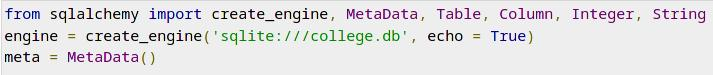
\includegraphics[width=\linewidth]{./images/connection.jpg}
  \vspace{.3cm}
  \caption{ Figure 3: Connection with database}
  \label{fig:Connection with database}
\end{figure3}

\subsection{Create Table}
We are creating a SQLite database college.db with a students table in it. The create\_all() function uses the engine object to create all the defined table objects and stores the information in metadata.
\item
\begin{figure4}
  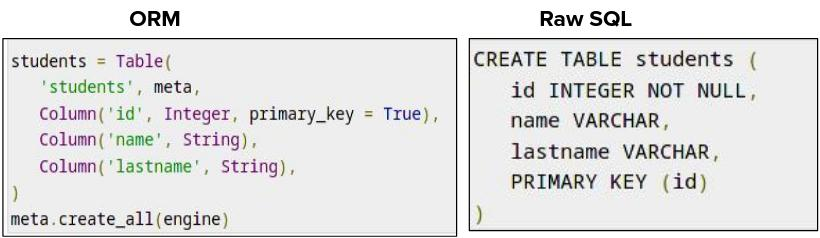
\includegraphics[width=\linewidth]{./images/create_table.jpg}
  \caption{Figure 4: Create table (ORM vs SQL)}
  \label{fig:Create table(ORM vs SQL)}
\end{figure4}

\subsection{Insert Data}
SQL expressions are constructed using corresponding methods relative to target table object. For example, the INSERT statement is created by executing insert() method as follows:
\item
\begin{figure5}
  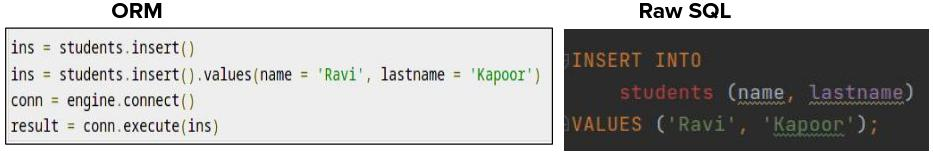
\includegraphics[width=\linewidth]{./imagees/insert.jpg}
  \caption{Figure: Insert data into database}
  \label{fig:Insert data into database (ORM vs SQL)}
\end{figure5}

\subsection{Print Data}
The select() method of table object enables us to construct SELECT expression. Using this we can print data from table.
\item
\begin{figure6}
  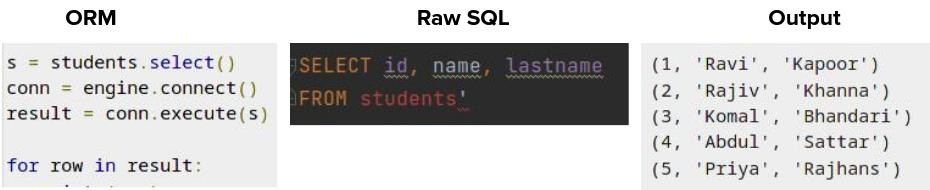
\includegraphics[width=\linewidth]{./images/select.jpg}
  \caption{Figure 6: Print data from database}
  \label{fig:Print data from database }
\end{figure6}

\subsection{Filter Data using 'Where'}
As similar to the SQL in ORM we have where() method to filter rows. so we can use it like this:
\item
\begin{figure7}
  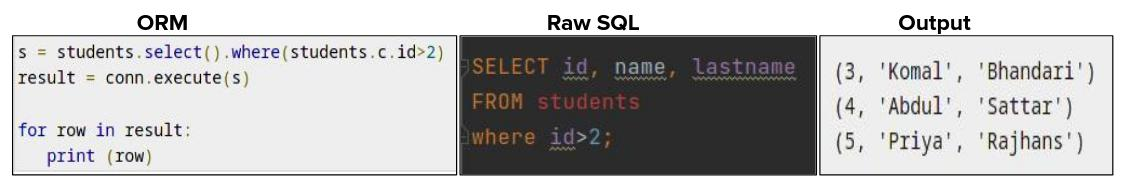
\includegraphics[width=\linewidth]{./images/where.jpg}
  \caption{ Figure 7:Print data from database with condition}
  \label{fig:Print data from database with condition (ORM vs SQL)}
\end{figure7}


\section{Features}
\begin{itemize}
\item It makes the application independent of the database management system being used in the backend, and so you can write a generic query. In case of migrating to another database, it becomes fairly a good deal to have ORM implemented in the project.
\item Hassles of coders are reduced to learn SQL syntaxes separately for whichever database being used to support the application. Coders can shift their focus on optimizing the code and improving performance rather than dealing with connectivity issues.
\item All small or big changes can be carried out via ORM, so there are no such restrictions when we deal with data. For example, JDBC comes with a lot of restrictions on extracting a result-set, process it and then commit it back to the database. This is not the case with ORMs. Even a single cell in the database can be retrieved, changed and saved back.
\item The connection becomes robust, secure as there will be less intervention in code. It will handle all the necessary configurations required to map application programming language with the database’s query language since there will be lesser intervention promoting secure application as a whole.
\item There is a fairly large deal of ORMs present in the market as per the application language used. One can choose easily as per business requirements.
\item There is an attached disadvantage in using ORM as well. That is when the database is in legacy file systems and disarranged. It becomes a task to arrange a whole lot of data and then map this with ORM. It is thereby suggested to use ORM when the back end is fairly managed.
\end{itemize}


\section{Pros of ORM}
\item ORM tools are popular with OOP developers because they minimize the amount of SQL knowledge required to connect a database to an application. ORMs also automatically generate the SQL code, allowing you to focus on generating business logic. There are four significant benefits of using object-related mappers to manage the interface between applications and databases.

\subsection{Productivity}
\item Writing data-access code is time-consuming and doesn’t add a lot of value to the application’s functionality. It’s essentially the plumbing of the code. Using a tool like an ORM that automatically generates the data-access code saves tremendous development time that does not add value to the application. In some cases, the ORM can write 100 percent of the data-access code for the application. The ORM can also help you keep track of database changes making it easier to debug and change the application in the future.

\subsection{Application Design}
A well-written ORM will implement design patterns to force you to use best practices for application design. If you use an ORM to manage the data interface, you do not need to create the perfect database schema in advance. You will be able to change the existing interface easily. Separating the database table from the programming code also allows you to switch out data for different applications.

\subsection{Code Reuse}
One way to reuse data is to create a class library to generate a separate dynamic-link library (DLL). You can create a new application without needing to duplicate the data-access code.

\subsection{Reduced Testing}
Since the code generated by the ORM is well-tested, you do not need to spend as much time testing the data-access code. Instead, you can focus on testing the business logic and code.


\section{Cons of ORM}
ORMs are an excellent tool for many applications, but some developers found several drawbacks in using ORMs for data-access applications. The issues seem to correlate with the complexity of the application. With simple applications, having a high-level of abstraction helps the development process. But when the applications are complex, abstraction covers up many details needed to address data-related issues.

\subsection{Performance}
A common complaint among OOP developers is the extra code generated by the ORM. The added code slows application performance and makes it harder to maintain. A well-designed ORM should be able to create high-quality code without affecting application speed.

\subsection{Need to Know SQL}
High-level abstractions do not always generate the best SQL code, and developers cannot rely on the ORM 100 percent of the time. You still need to know SQL as well as the syntax generated by the ORM.

\subsection{Poor Mapping}
ORMs can sometimes create an incorrect mapping between data tables and objects. These problems can cause application problems and be difficult to recognize. ORMs also encourage one-to-one mapping even though it is rare that business applications have many one-to-one relationships.


\section{Conclusion}
Writing SQL code to attach a relational database to an object-oriented application can be a time-consuming activity that generates little value to the business application. Developers can write raw SQL code or use SQL query builders to improve the process, but both methods still require in-depth database knowledge and the ability to code in SQL. ORMs enhance productivity by creating highly-abstract data models and automatically generating SQL code. These tools also make it easier to separate the database from the programming logic giving developers more flexibility. But ORMs have their detractors. Common complaints include reduced performance, extra coding, and poor mapping depending on the ORM quality.


\section{Reference}
\begin{enumerate}
\item https://www.altexsoft.com/blog/object-relational-mapping/
\item http://www.diva-portal.org/smash/get/diva2:1014983/FULLTEXT02
\item https://www.educba.com/what-is-orm/
\end{enumerate}

\end{document}
